%%%%%%%%%%%%%%
% ch3 : cristallographie % 
%%%%%%%%%%%%%%

\chapter{L'état cristallin et l'état amorphe}
\section{Introduction}
	\begin{wrapfigure}[6]{l}{5cm}
	\vspace{-6mm}
	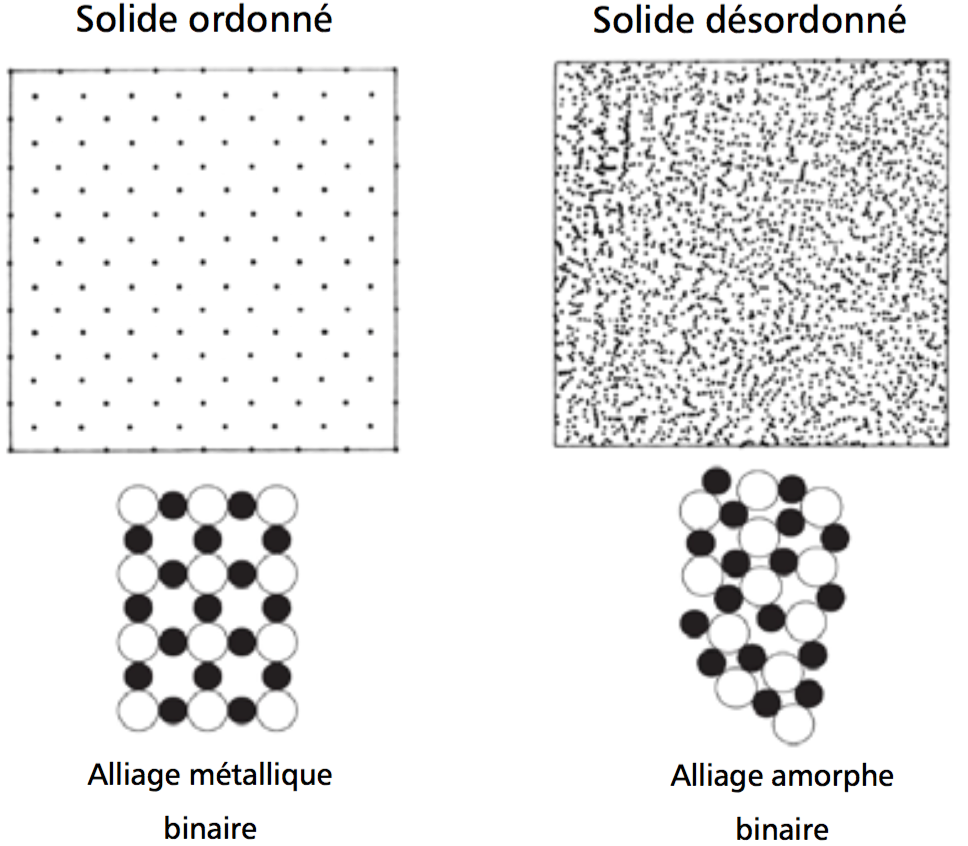
\includegraphics[scale=0.28]{ch3/1}
	\end{wrapfigure}
	Un solide cristallin (ordonné) est caractérisé par un ordre sur de longues distances alors qu'un solide amorphe (désordonné) ou vitreux se caractérise par l'absence d'ordre. Les métaux et les céramiques sont cristallins. Des températures de refroidissement extrêmes depuis l'état fondu peuvent donner lieu à des métaux amorphes pour des alliages assez complexes.\\\\\\
	
	\begin{wrapfigure}[6]{r}{3cm}
	\vspace{-10mm}
	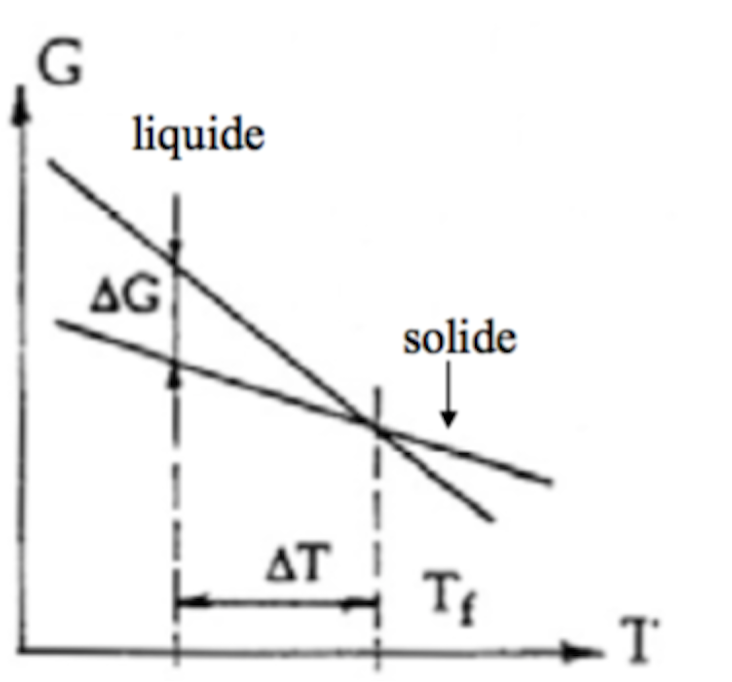
\includegraphics[scale=0.25]{ch3/2}
	\end{wrapfigure}
	La thermodynamique nous apprend qu'à pression constante, l'état d'équilibre correspond au minimum de l'\textbf{enthalpie libre de Gibbs}
	\begin{equation}
		G = H-TS
	\end{equation}
	On sais alors qu'à \textbf{haute température}, l'enthropie du liquide étant plus grande que celle du solide (plus de désordre dans le liquide), la composante enthropique va l'emporter et le liquide aura une énergie libre plus faible $\rightarrow$ stable.\\
	Au contraire, à basse température, c'est l'enthalpie qui prend le dessus et est lié au rassemblement des molécules sous l'effet des forces de liaison qui entraîne sa diminution $\rightarrow$ solide.\\
	 A une température $T_f$, l'énergie des deux phases sont égales, c'est la température de fusion. 
	 
	\begin{wrapfigure}[7]{l}{3.7cm}
	\vspace{-5mm}
	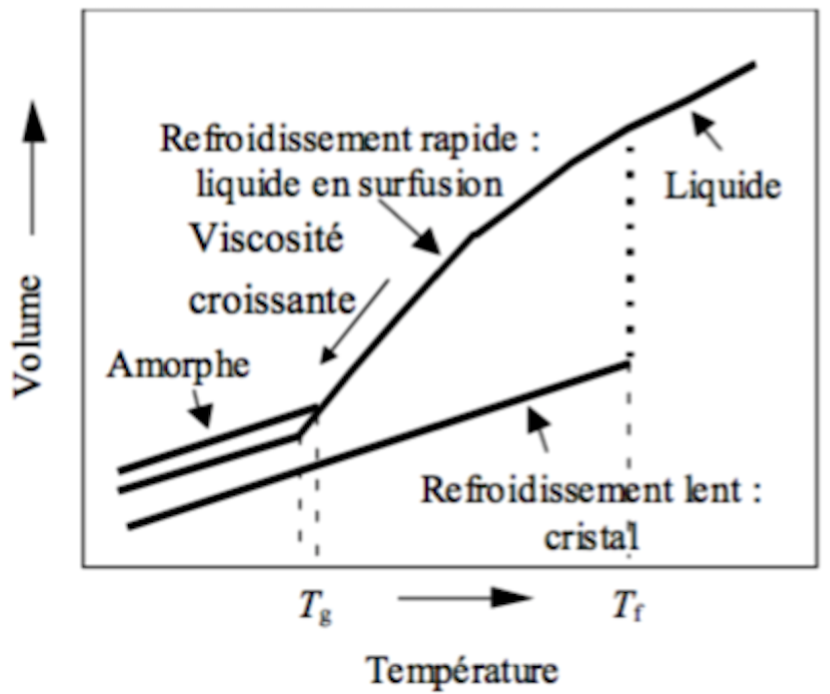
\includegraphics[scale=0.25]{ch3/3}
	\end{wrapfigure}
	En refroidissant lentement un liquide, on observera à la température de fusion une contraction du volume qui traduit la \textbf{mise en ordre} des atomes. Ils adoptent un empilement ordonné bien plus compact de manière à produire l'enthalpie de liaison (négative) la plus grande. Le solide sera à l'état \textbf{cristallin}.\\
	
	Lorsque la vitesse de refroidissement augmente, la contraction démarre à une \textbf{température plus basse.} Pour les longues chaînes polymétriques ou des silicates complexes (systèmes complexes), la forme stable est une forme cristalline à basse température, mais la mise en place est tellement complexe qu'un refroidissement rapide l'en empêche. Dans ce cas, lorsque la température diminue, la viscosité du liquide augmente et peut aller jusqu'à une température en dessous de laquelle l'agitation thermique n'est plus suffisante pour permettre le mouvement des atomes. Le liquide se fige alors et forme un solide en gardant la structure désordonnée du liquide $\rightarrow$ \textbf{amorphe}. La température à laquelle le liquide se fige est appelé \textbf{température de transition vitreuse} $\mathbf{T_g}$.
	
\section{Les cristaux métalliques}
		\subsection{Structures compactes}
			Lorsque la cohésion n'est assuré que par des liaisons non-directionnelles comme la liaison métallique idéale, le minimum d'énergie s'obtient quand on a l'empilement la plus compact (ions positifs + gaz d'électrons). Dans les solides métalliques, la taille des ions métalliques dépend de la taille de leurs orbitales électroniques internes qui ne participent pas à la liaison. A partir d'une certaine distance, l'interpénétration de ces orbitales provoque une force de répulsion augmentant très abruptement. \\
			
			\begin{wrapfigure}[5]{r}{3.2cm}
			\vspace{-5mm}
			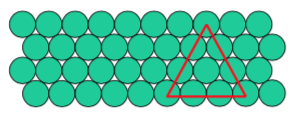
\includegraphics[scale=0.7]{ch3/4}
			\end{wrapfigure}
			On peut donc assimiler les ions à des sphères dures en contact. On peut voir ci-contre le moyen de former la structure la plus compacte avec des sphères. Cela s'appelle un \textbf{plan compact} et les lignes rouges représentent les directions compactes (directions selon lesquelles les sphères se touchent).\\
			
			\begin{wrapfigure}[4]{l}{3.1cm}
			\vspace{-7mm}
			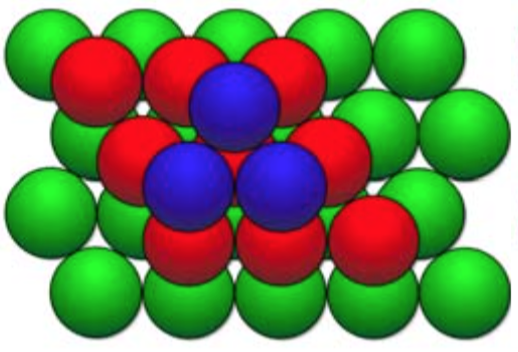
\includegraphics[scale=0.32]{ch3/5}
			\end{wrapfigure}
			Les empilements tridimensionnels les plus compacts s'obtiennent par empilement de plans compacts les uns sur les autres. Nommons le premier plan "A" et le deuxième "B", le B va venir se placer dans les interstices entre les sphères du A. Il existe alors 2 familles de sites au-dessus desquels le second plan peut venir se placer. Ceci est montrer sur le schéma ci-contre. Ce même schéma montre comment se disposerait un troisième plan sur le précédent. 
			
			\begin{wrapfigure}[4]{r}{2.8cm}
			\vspace{-8mm}
			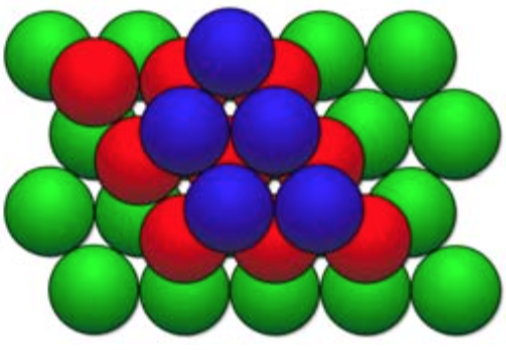
\includegraphics[scale=0.32]{ch3/6}
			\end{wrapfigure}
			De nouveau, il a le choix entre deux familles d'emplacements : position des ions A ou l'autre. Ici est représentée justement la disposition "ABABA" où le troisième plan est à la position du plan A en hauteur. Le schéma précédent représente le cas "ABCABC. Selon les deux empilements présentés, on obtiendra deux structures cristallines différentes et sont appelées \textbf{structures compactes}. Ce sont les deux seules manières d'empilement vérifiant la condition de compacité.
			La "ABCABC" donne naissance à la structure \textbf{cubiques à faces centrées (CFC)} et la "ABAB" à la structure \textbf{hexagonales compacte (HC)}.
			
		\subsection{La structure cubique faces centrées}
			\begin{wrapfigure}[5]{l}{5cm}
			\vspace{-5mm}
			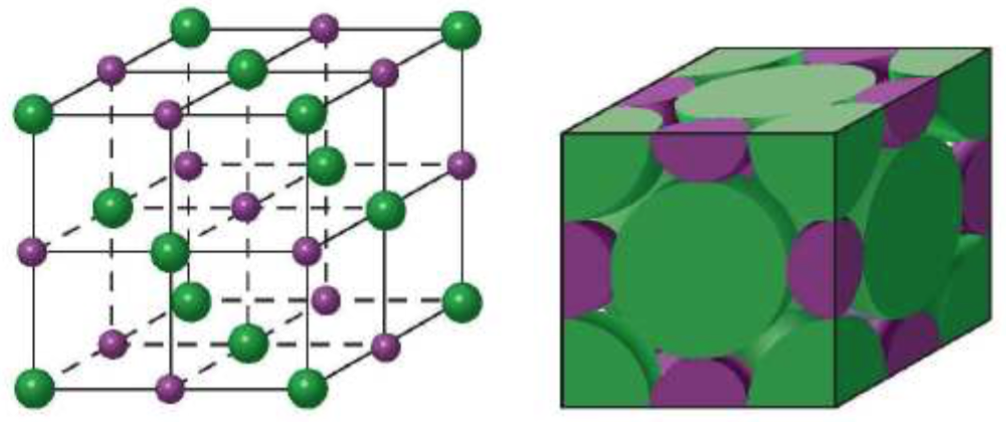
\includegraphics[scale=0.9]{ch3/7}
			\end{wrapfigure}
			Les fameux plans compactes correspondent aux plans diagonaux passant par trois sommets d'un cube élémentaire possédant un atome à chaque sommet et un atome au centre de chaque face. C'est cette géométrie qui donne le nom de cubique faces centrées. Les directions compactes des plans compactes correspondent aux diagonales des faces. Le cube possède 4 plans diagonaux. Ceci signifie qu'on peut construire le même cristal en empilant des plans compacts suivant 4 directions différentes (grand degré de liberté). \\
			Chaque sphère est en contact avec 12 voisins immédiats, on dit que le nombre de coordination des ions est égal à 12. Le nombre d'atomes présents dans le cube est de 4 car 8/8+6/2 = 4.\\
			
			\subsubsection{Compacité}
			\begin{wrapfigure}[5]{l}{3.3cm}
			\vspace{-5mm}
			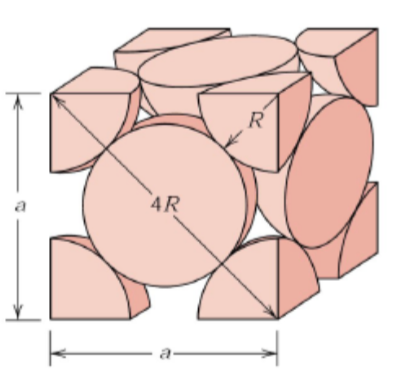
\includegraphics[scale=0.5]{ch3/8}
			\end{wrapfigure}
			Calculons la compacité qui représente la proportion de l'espace rempli par les sphères en contact. Elle est défini comme\footnote{APF = Atomic Packing Factor, FCC = Face Cubique Centré}
				\begin{equation}
					APF_{FCC} = \frac{\mbox{volume total de la sphère}}{\mbox{volume du cube}} = \frac{4\left( \frac{4}{3}\pi R^3 \right)}{a^3}					
				\end{equation}					
				où $a$ est déterminé par le théorème de pythagore
				\begin{equation}
					a^2+a^2 = (4R)^2 \qquad \Rightarrow \qquad a = 2R\sqrt{2}
				\end{equation}
				De ce fait, la compacité est donné par 
				\begin{equation}
					APF_{FCC} = \frac{\frac{16}{3}\pi R^3}{16R^3\sqrt{2}} = 0.74 = APF_{HC}
				\end{equation}
				et est la même pour la structure hexagonale compacte !
		\subsection{La structure hexagonale compacte}
			\begin{wrapfigure}[6]{r}{2.8cm}
			\vspace{-5mm}
			
\includegraphics[scale=0.5]{ch3/9}
			\end{wrapfigure}
			Dans ce cas, les atomes se répartissent selon un prisme hexagonal où les plans compactes correspondent aux plans des deux bases ainsi qu'à un plan parallèle à mi hauteur. On a de ce fait un atome à chaque sommet, un au centre des bases et trois formant un triangle à mi-hauteur. Il n'existe cette fois qu'une famille de plans compacts et orientés parallèlement à la base du prisme (degré de liberté plus faible). \\
			Les 3 directions compactes sont suivant les arêtes de la base du prisme. La longueur des arêtes est désigné par "$a$" et celle des hauteurs par "$c$". Si les billes sont en contact, on calcule que le rapport $c/a$ doit être égal à 1.623. Tout écart par rapport à cette valeur signifie que la liaison n'est pas à 100\% métallique (jamais observé).
			
		\subsection{La structure cubique centrée}
			On peut s'attendre avec ce qu'on a vu à ce que les métaux ayant une structure CFC soient ceux dont la cohésion est dû à la liaison métallique la plus pure. En effet, les métaux nobles, le nickel, l'aluminium et les gaz nobles cristallisés à très basse température (car non-directionnalité des forces de Vander-Waals) adoptent une structure CFC. \\
			Ceux qui adoptent la structure HC sont le magnésium, le zinc et le cadmium. Ces éléments présentent un caractère métallique moins parfait que les métaux alcalins et nobles. 	\\
			Les métaux alcalins présentent une structure CFC qu'à basse température. A l'ambiante, l'agitation thermique fait qu'ils sont moins compactes $\Rightarrow$	\textbf{la structure cubique centrée}. 1/3 des métaux purs présentent une structures différentes des deux présentées. L'enthalpie libre de ces métaux est plus élevé dans le cas compact que dans le cas moins compact. Ceci est dû à  deux effets : 
			\begin{itemize}
				\item[•] une contribution de la liaison covalente peut imposer une certaine directionnalité de liaison difficilement compatible avec l'empilement compact;
				\item[•] l'entropie étant plus élevé dans le cas moins compacte, l'élévation de la température peut donner lieu à une structure plus stable que le compact. 
\end{itemize}		
			
			\begin{wrapfigure}[5]{l}{5cm}
			%\vspace{-5mm}
			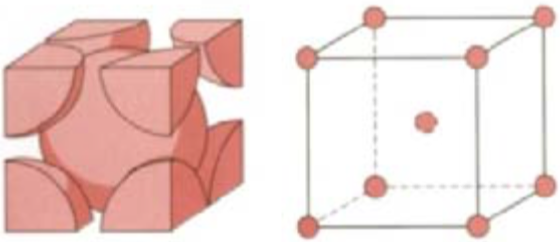
\includegraphics[scale=0.5]{ch3/10}
			\end{wrapfigure}
			La structure non compacte la plus courante est la cubique centrée. Le cube contient un atome aux 8 sommets ainsi qu'un au centre. Ce n'est pas une structure compacte, le taux de remplissage est de 68\%. Chaque atome ne compte que 8 voisins au lieu de 12 et la direction la plus compacte est la diagonale du cube. La majorité des métaux de transition présentent cette structure en raison du caractère partiellement covalent de la liaison dû à la participation des couches $d$ incomplètes. 
			
		\subsection{Transformation allotropiques : le cas du fer}
			De nombreux solides présentent des "variétés allotropiques", c'est à dire des structures cristallines différentes à différentes températures. L'enthalpie dépend ainsi de la température (ou de la pression). Ce phénomène est appelé \textbf{transformation allotropique}. Le fer par exemple, à pression constante, est CC jusque $912\degres C$, CFC de $912\degres C$ à $1394\degres C$ et CC au delà. \\
			Lors d'un refroidissement, la première transformation de CC vers CFC se fait à $1394 \degres C$ et résulte de la plus faible enthropie du CFC. On désigne cette variante du fer \textbf{austénite} ou $Fe\gamma$. \\
			La seconde transformation résulte de la diminution de l'enthalpie libre du CC en raison de l'apparition du ferromagnétisme dans cette structure traduisant une diminution de l'entropie. Le ferromagnétisme n'apparaît que dans le CC et pleinement en dessous de la \textbf{température de Currie} qui se situe à $770\degres C$ pour le fer C. On désigne cette structure CC de \textbf{ferrite} ou $Fe \alpha$.
			
\section{Les cristaux ioniques}
	\begin{wrapfigure}[5]{r}{5.4cm}
	\vspace{-5mm}
	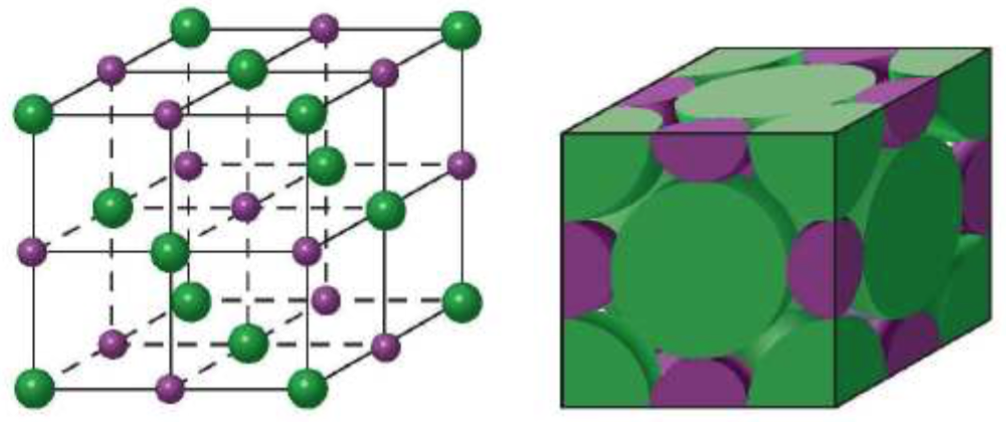
\includegraphics[scale=0.3]{ch3/11}
	\end{wrapfigure}
	Ils sont constitués d'un empilement d'ions de charge différente. Ceux-ci doivent s'empiler de la manière la plus compacte possible pour avoir une enthalpie libre minimale, en tenant compte de leur taille et de la neutralité des charges électriques. Ci-contre est présenté l'exemple du $NaCl$ où les anions $Cl^-$ sont plus volumineux que les cations. On peut voir ça comme deux structures CFC imbriquées où les cations viennent se mettre dans les interstices de la structure des anions. Chaque ion est en contact avec 6 contre-ions (nombre de coordination). 

\section{Les cristaux covalents}
	\begin{wrapfigure}[5]{l}{2.8cm}
	\vspace{-5mm}
	
\includegraphics[scale=0.5]{ch3/9}
	\end{wrapfigure}	
	La géométrie des solides covalents est essentiellement dictée par a directionalité de la liaison, menant à des structures très ouvertes et peu compactes. Ci-contre, l'hybridation $sp3$ des orbitales du carbone sous forme de diamant impose un angle de $109.5\degres C$ entre les liaisons, faisant tomber le nombre de coordination à 4 et la compacité à 0.34 (2x moins que CFC et HC).
	
\section{La structure des polymères}
	\subsection{Quelques polymères courants}
		\begin{wrapfigure}[2]{r}{3.2cm}
		\vspace{-5mm}
		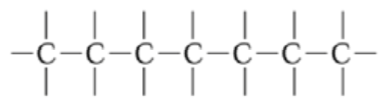
\includegraphics[scale=0.5]{ch3/9p}
		\end{wrapfigure}	
		Les polymères sont formés de très grosses molécules pouvant compter plusieurs centaines de milliers d'atomes. Le mot "polymère" vient du grec "poly" signifiant plusieurs et "meros" partie ou unité. Ces unités de répétitions sont appelés \textbf{monomères} et sont des molécules organiques dont le noyau est essentiellement constitué d'un atome de \textbf{carbone}. Dans une même chaine, les liaisons sont fortes (covalentes C-C) alors qu'entre macromolécules, les liaisons sont faibles (secondaires).
	\subsection{Polymérisation en chaîne}
	\subsection{Masse molaire moyenne et distribution}
	\subsection{Configuration géométrique}
	\subsection{Classification}
	\subsection{Propriétés}
	
